\documentclass[12pt, a4paper]{article}

\usepackage[brazilian]{babel}
\usepackage[T1]{fontenc}
\usepackage{amsmath}
\usepackage{graphicx}
\usepackage{float}
\usepackage[top=3cm,bottom=3.5cm,left=3.5cm,right=3.5cm,marginparwidth=1.75cm]{geometry}
\usepackage[hidelinks, bookmarksnumbered=true]{hyperref}

\begin{document}

\phantomsection
\addcontentsline{toc}{section}{Folha de rosto}
% --------------
% Folha de Rosto
% --------------
\pagestyle{empty}	% Folha de rosto e apresentação não mostram a numeração.


\begin{flushleft}
    \parbox{2.5cm}{
\includegraphics[width=2.3cm]{PEF_minerva.pdf} }
    \parbox{10cm}{
        UNIVERSIDADE FEDERAL DO RIO DE JANEIRO \\ 
        Instituto de Física \\ 
        Programa de Pós-Graduação em Ensino de Física \\ 
        Mestrado Profissional em Ensino de Física}
\end{flushleft}

\begin{center}
\vspace{2cm}
{\large\textbf{\Large Medidas e Incertezas}} % Título do material


% 1ex é a altura de uma letra x na fonte usada.
\vspace{0.5cm}
\begin{flushright}
    \parbox{9cm}{ \large
        {Caio M. Ferreira      \\
        Carlos Eduardo Aguiar  \\
        Roberto A. Pimentel Jr \\
        Gustavo M. Rubini}}        % Autores
\end{flushright}
\end{center}

\vspace{1.5cm}
\begin{flushright}
    \parbox{10.7cm}{\large
    Material instrucional apresentado ao Programa de Pós-Graduação em Ensino de Física, do Instituto de Física da Universidade Federal do Rio de Janeiro, como parte dos requisitos necessários à obtenção do título de Mestre em Ensino de Física.
    }
\end{flushright}

\vfill

\begin{center}
Rio de Janeiro\\Dezembro de 2024
\end{center}

\newpage

%--------------------
% Apresentação
%--------------------

\vspace*{2cm}

\noindent \textit{Cara professora, caro professor}: \medskip

O texto apresentado a seguir, \emph{Medidas e Incertezas},  introduz noções básicas sobre a obtenção e análise de dados experimentais por meio de uma sequência de atividades desenvolvidas para estudantes do ensino médio. As atividades envolvem medidas do tempo de reação dos alunos a  estímulos visuais, realizadas com auxílio de um aplicativo criado especialmente para essa finalidade, que pode ser acessado de qualquer \emph{smartphone} ou computador.
A importância de se realizar várias medições é discutida durante as atividades, assim como maneiras de sistematizar e apresentar os resultados encontrados. Nesse processo, construtos como o histograma são apresentados e os conceitos de valor médio e incerteza das medidas são expostos sem recorrer a formulações matemáticas elaboradas, de modo a enfatizar seu significado intuitivo.
O papel da incerteza em qualquer processo de medida é ressaltado, mostrando como é essencial avaliar quantitativamente a confiabilidade de um resultado experimental para que se possa tomar decisões baseadas nele.

Na escola, as atividades e discussões propostas podem ser realizadas em dois tempos de aula de 50 minutos cada. O texto disponível aqui pode ser utilizado tanto pelo professor, como um roteiro para as aulas, quanto pelos alunos, como material de estudo e aprofundamento.

Mais informações sobre o ensino de mensuração e incerteza podem ser encontrados na dissertação de mestrado de Caio Ferreira, \emph{Medição, Incerteza e Evidência Empírica}, em {\small \url{http://pef.if.ufrj.br/producao_academica/dissertacoes/2024_Caio_Ferreira/dissertacao_Caio_Ferreira.pdf} }.

\newpage

% -------------------------------
%  Texto principal
%--------------------------------

\setcounter{page}{1} % Começa a contar páginas
\pagestyle{plain}	     % Folhas numeradas

\begin{center}
\textbf{\Large Medidas e Incertezas}
\end{center}

\section{Introdução}

Imagine a situação em que precise conhecer a maior massa que pode ser suportada por um barbante preso ao teto, sem que ele se rompa. Para medir esse valor penduramos no fio massas cada vez maiores, até que ele arrebente. Vamos supor que o barbante suportou todas as massas até 410~g, mas rompeu-se quando a massa suspensa foi aumentada para 420~g. Com o rompimento, temos uma medida da massa limite suportada pelo fio, mas será que conhecemos bem esse limite? O que aconteceria se pendurássemos, por exemplo, uma carga de 414~g? E o que é mais importante, se utilizarmos outra amostra do mesmo tipo de barbante (afinal, a primeira foi arrebentada), ela também seria rompida entre 410~g e 420~g? Podemos ter certeza que ela aguentaria 400~g, por exemplo? Ou que seria rompida por 430~g?

Em situações como a descrita acima, devemos avaliar com cuidado a confiança que temos no resultado da medição, ou seja, é necessário estimar a incerteza associada à medida. É impossível medir exatamente a massa limite para o rompimento de uma dada amostra de um determinado tipo de fio. Entretanto, é possível elaborar o quanto de confiança podemos depositar na medida desse limite e buscar formas de ter mais segurança em nossas medições.

Esta questão ocupa todas as ciências: o tamanho das peças do motor de um carro, a eficácia de um medicamento, o produto interno bruto de um país, todas essas medidas possuem o que chamamos de \textbf{incerteza de medição}. Contudo, apesar de possuírem incertezas, elas desempenham papéis fundamentais em nossa sociedade. Isso acontece porque a incerteza de cada medida é algo calculável, e nos fornece o próprio grau de confiança que podemos ter na medida.

Neste texto vamos discutir a realização de medições, como representar seus resultados, como calcular incertezas e como utilizar tudo isso para fazer comparações e tomar decisões. Faremos isso usando como exemplo a medida do tempo de reação de uma pessoa. Essa medição pode ser realizada em sala de aula ou em casa com um aplicativo desenvolvido para este fim. O mesmo aplicativo permite a análise da incerteza associada ao resultado obtido.

\section{Tempo de reação}

Ao dirigir um veículo, é importante que o tempo de reação do condutor seja pequeno, para que, caso ocorra algum imprevisto, ele possa reagir o mais rápido possível. O tempo de reação também é relevante para situações esportivas, desde a largada em uma prova de corrida, até a defesa de um pênalti em uma partida de futebol. 
Existem ao menos três categorias de tempo reação, baseados em diferentes tipos de estímulo: auditivo, tátil e visual. As medições que iremos considerar são do tempo de reação a um estímulo visual.

\section{Coleta e apresentação de dados}
\subsection{Medição do tempo de reação}

Existem várias formas de fazer a medição do tempo de reação. Nós utilizaremos um aplicativo que simplifica bastante essa medição e organiza os dados em uma forma gráfica que nos permite entender melhor os resultados encontrados.

O aplicativo pode se usado a partir de qualquer celular ou computador conectado à internet. Ele é executado em {\small \url{http://pef.if.ufrj.br/producao_academica/dissertacoes/2024_Caio_Ferreira/tempo-reacao/tempo.html} }. Ao acessar essa página, pode-se ver uma área cinza contendo o botão ``Fazer medida'', como mostrado na figura~\ref{abertura}.

\begin{figure}[!hbt]
\centering
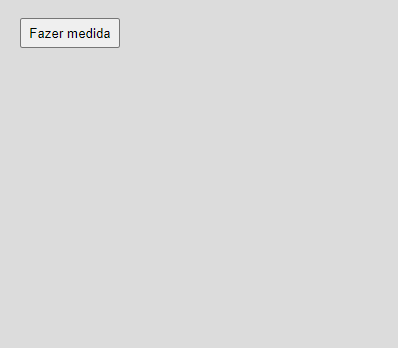
\includegraphics[width=0.35\linewidth]{app1.png}
\caption{Aspecto inicial do aplicativo.}
\label{abertura}
\end{figure}

Quando esse botão é acionado, surge uma mensagem “Clique na tela quando a cor mudar”. Após um intervalo escolhido ao acaso pelo aplicativo, a área cinza muda de cor. O aspecto do aplicativo antes e logo depois desse intervalo está na figura~\ref{iniciado}.

\begin{figure}[!hbt]
    \centering
    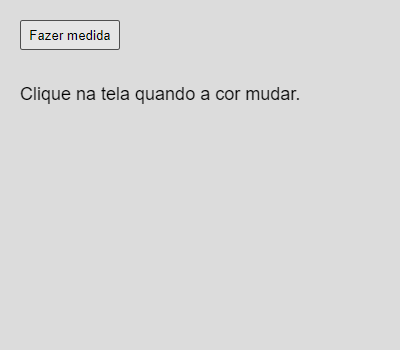
\includegraphics[width=0.35\linewidth]{app2.png}
    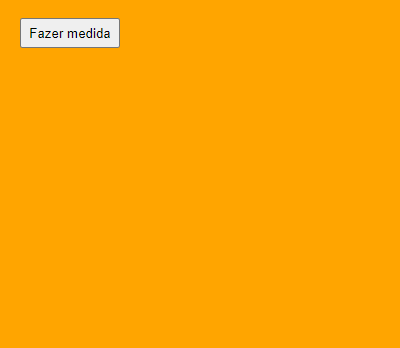
\includegraphics[width=0.35\linewidth]{app3.png}
    \caption{ Aplicativo iniciado.}
    \label{iniciado}
\end{figure}

No instante da mudança de cor da tela, inicia-se uma contagem de tempo, que será interrompida por um toque na tela do celular ou clique do mouse na área laranja. O tempo entre a mudança de cor e o toque ou clique é o tempo de reação da pessoa, que será escrito na tela como se vê na medida mostrada na figura~\ref{uma_medida}. A unidade de tempo utilizada é o segundo (abreviado como s).

\begin{figure}[H]
\centering
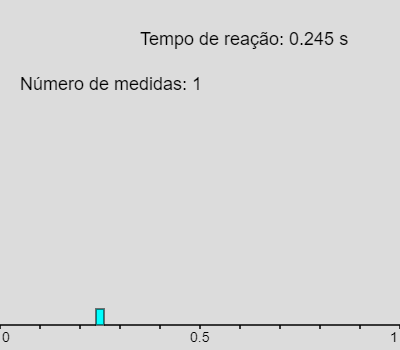
\includegraphics[width=0.52\linewidth]{new app4.png}
\caption{Medida do tempo de reação realizada com o aplicativo. O resultado é indicado numericamente e também pela posição de uma caixa sobre o eixo de tempo, que vai de 0 a 1~s em intervalos de 0,1~s.}
\label{uma_medida}
\end{figure}

Além de registrar o valor do tempo de reação, o aplicativo desenha uma caixa azul que representa a medida em um eixo de tempo que vai de 0,0 a 1,0~s. Note que essa caixa tem uma certa largura, dentro da qual está o valor medido. No caso a medida foi 0,245~s e a caixa vai de 0,24~s a 0,26~s, ou seja, sua largura é 0,02~s. 


\subsection{Medidas e histograma}

Com o valor que obtivemos (0,245~s), \textbf{podemos afirmar que conhecemos o tempo de reação da pessoa que realizou a medição?}
Para verificar se a afirmativa é correta, a mesma pessoa faz outra medição com o aplicativo. O resultado está mostrado na figura~\ref{duas_medidas}.

\begin{figure}[H]
\centering
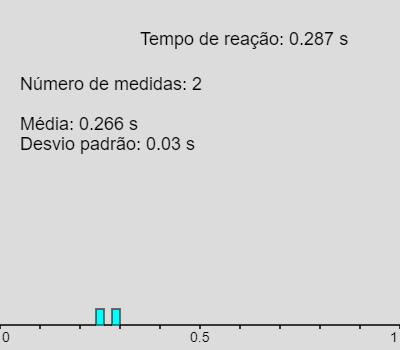
\includegraphics[width=0.52\linewidth]{new app5.png}
\caption{ Duas medidas coletadas.}
\label{duas_medidas}
\end{figure}

Na segunda medição, há um valor diferente para o tempo de reação, 0,287~s, em vez da repetição do primeiro valor 0,245~s. O aplicativo mostra em sua tela o tempo que acaba de ser medido, o número de medidas já realizadas e outras informações -- a média e o desvio padrão -- cujo significado discutiremos mais à frente. Além disso, mais uma caixa azul é colocada sobre o eixo, representando a nova medida. Vemos que há uma diferença perceptível entre as duas medidas, mas alguma delas é melhor que a outra? 

As duas foram realizadas corretamente pelo mesmo processo, portanto não há motivos para escolhermos apenas uma como o tempo de reação, excluindo a outra. Para compreender melhor o que está acontecendo, vamos realizar mais oito medidas, completando um total de dez. Os resultados estão mostrados na tabela~\ref{tab:widgets}.

\begin{table} [H]
\centering
\begin{tabular}{l|r}
Medida & Valor (s) \\\hline
1 & 0,245 \\
2 & 0,287 \\
3 & 0,266 \\
4 & 0,264 \\
5 & 0,257 \\
6 & 0,274 \\
7 & 0,236 \\
8 & 0,284 \\
9 & 0,276 \\
10 & 0,260\\
\end{tabular}
\caption{\label{tab:widgets}Tabulação das medidas.}
\end{table}

Não é fácil perceber a partir da tabela como os resultados estão distribuídos. Uma forma de facilitar essa análise está na figura \ref{fig:app6}, que mostra a tela do aplicativo ao final das dez medidas. Na parte de baixo dessa figura está o que chamamos de \textbf{histograma} dos resultados. Esse histograma é construído a partir da divisão do eixo horizontal em intervalos de $0,02$~s, assim temos: 0,00 a 0,02, de 0,02 a 0,04, de 0,04 a 0,06... Cada medida do tempo de reação é marcada no intervalo que a contém, no gráfico, colocando sobre esse intervalo uma caixa, como vimos na figura~\ref{uma_medida}. Caso uma nova medida seja encontrada em um intervalo já ocupado por uma medida prévia, a caixa da nova medida será empilhada sobre a anterior. Com mais medidas, surgem torres de caixas empilhadas, indicando a ocorrência de várias medidas no intervalo. Esse tipo de gráfico é útil para visualizar e comparar a frequência com que eventos acontecem em cada faixa.

\begin{figure}[H]
\centering
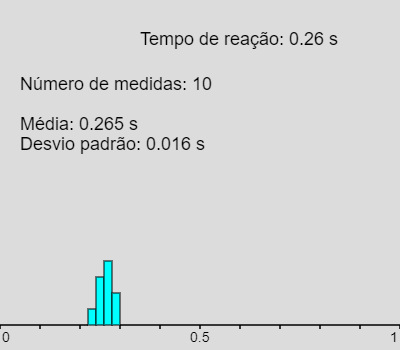
\includegraphics[width=0.55\linewidth]{new app6.png}
\caption{\label{fig:app6} Histograma das dez medidas. Note como o histograma é mais útil para visualizar a distribuição das medidas do que a tabela~\ref{tab:widgets}.}
\end{figure}

Em virtude da variação do valor do tempo de reação nas diferentes medições, torna-se difícil escolher uma determinada medida para descrevê-lo. Todavia, podemos utilizar a \textbf{média} de todas as medidas realizadas (0,265 segundos) para obter uma representação do tempo de reação que leve em consideração a informação que está disponível.

\section{A representação pela média}

A média de um conjunto de $n$ números, $x_1, x_2, x_3, ...$, é definida como:

\[\boxed{\Bar{x} = \frac{x_1 + x_2 + \cdots + x_n}{n}}\, .\]
No caso de $n$ medidas de tempo de reação, como as discutidas acima, aplicando essa definição encontraríamos o tempo de reação médio. 

\[\Bar{t} = \frac{t_1 + t_2+...+t_n}{n}\]
Por exemplo, a média das duas medidas ilustradas na figura~\ref{duas_medidas} é:

\[\Bar{t}=\frac{0,245+0,287}{2}=0,266\, .\]
Essa média foi calculada pelo aplicativo e escrita na tela, como também se vê na figura \ref{duas_medidas}. Note que a média ficou bem no meio entre as duas medidas. Para dez medidas, como na figura~\ref{fig:app6}, temos o seguinte:

\[
\Bar{t} = \frac{0,245+0,287+0,266+\cdots+0,284+0,276+0,260}{10} 
          = 0,2649
\]
Da mesma forma que em $n=2$, a média das dez medidas é calculada pelo aplicativo, conforme mostrado na figura \ref{fig:app6}.  Ela é escrita com o mesmo número de casas decimais das medidas; por isso o programa arredonda 0,2649 para 0,265. A média representa razoavelmente bem o valor típico das medidas, mesmo que nenhuma medição tenha encontrado esse valor. A figura \ref{histograma princ} mostra o histograma das dez medidas com a média indicada no eixo horizontal. Vemos que o valor médio dá uma boa indicação sobre os tempos de reação encontrados.

\begin{figure}[H]
    \centering
    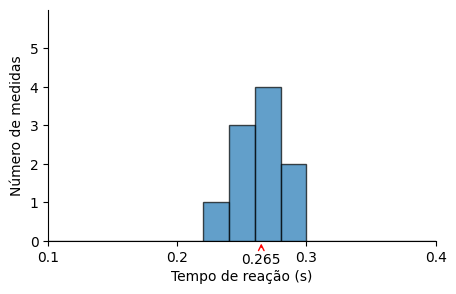
\includegraphics[width=0.55\linewidth]{histograma princ..png}
    \caption{A seta indica a localização da média no histograma das 10 medidas.}
    \label{histograma princ}
\end{figure}


\section{Dispersão das medidas e desvio-padrão}

Embora a média dê uma boa descrição do conjunto de medidas, ela não diz nada sobre a dispersão dos valores encontrados em cada medição. A dispersão das medidas do tempo de reação indica como a resposta da pessoa a um estímulo varia de uma medição para outra. Medidas próximas umas das outras indicam que as reações são sistematicamente semelhantes, enquanto medidas muito espalhadas apontam para respostas pouco consistentes entre si. Na figura~\ref{consistência}, há dois histogramas de medidas do tempo de reação obtidos por pessoas diferentes. As medidas do histograma da esquerda (obtidos pela pessoa \textit{A}) estão mais dispersas que as medidas do histograma à direita (obtidos pela pessoa \textit{B}).

\begin{figure}[H]
    \centering
    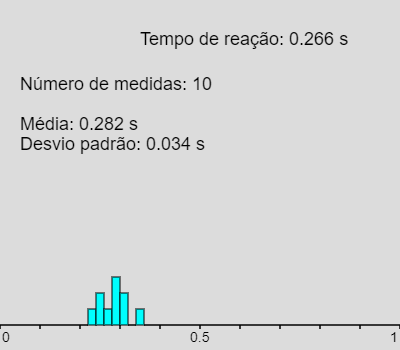
\includegraphics[width=0.4\linewidth]{app7.png}~
    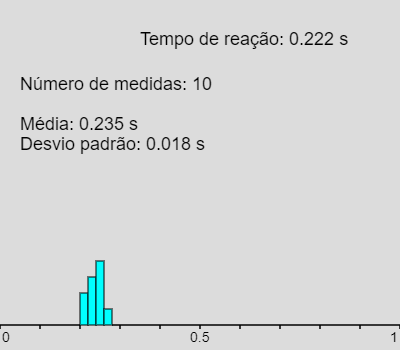
\includegraphics[width=0.4\linewidth]{app8.png}
    \caption{ Histograma da pessoa~\textit{A} à esquerda e da pessoa~\textit{B} à direita.}
    \label{consistência}
\end{figure}

A largura do intervalo ocupado pelo histograma dá uma ideia de como as medidas estão dispersas em torno de sua média. Quantitativamente, o grau dessa dispersão costuma ser representado pelo \textbf{desvio-padrão}.

Para calcular o desvio padrão, adotamos o seguinte procedimento. Começamos calculando os desvios de cada medida em relação à média,

\[\text{desvios: } (t_1-\Bar{t}), \, (t_2-\Bar{t}), \, \dots \, (t_n-\Bar{t})\, .\]
Como alguns desvios serão positivos e outros negativos, elevamos cada um ao quadrado, para obter sempre números positivos, e os somamos:

\[(t_1-\Bar{t})^2 +(t_2-\Bar{t})^2 + \ldots + (t_n-\Bar{t})^2\, .\]
De maneira semelhante à média, dividimos o resultado da soma pelo número de elementos envolvidos, obtendo

\[\frac{(t_1-\Bar{t})^2 +(t_2-\Bar{t})^2 + \ldots + (t_n-\Bar{t})^2}{n}\, .\]
Observe que se tivéssemos tomado a média dos desvios o resultado seria zero, pois os desvios negativos cancelariam os positivos. Como estamos interessados no tamanho dos desvios, e não para qual lado da média eles foram, tomar seu quadrado elimina essa distinção. Como o resultado é a média do quadrado dos desvios, o tamanho típico do desvio será a raiz quadrada dessa média, ou seja,

\[\sqrt{\frac{(t_1-\Bar{t})^2 +(t_2-\Bar{t})^2 + \ldots + (t_n-\Bar{t})^2}{n}}\, .\]
É costumeiro substituir o $n$ no denominador por $n-1$, definindo o desvio-padrão, que chamaremos de $\sigma$, por

\[\boxed{\sigma=\sqrt{\frac{(t_1-\Bar{t})^2 +(t_2-\Bar{t})^2 + \ldots + (t_n-\Bar{t})^2}{n-1}}}\, .\]
Existem justificativas para colocar esse $n-1$ no denominador. De maneira simplista, podemos dizer que ele indica a impossibilidade de calcular o desvio-padrão de apenas uma medida, pois isso resultaria em uma divisão de zero por zero na fórmula acima.

Como exemplo, abaixo está o cálculo do desvio-padrão das duas medidas presentes na figura~\ref{duas_medidas}:

\[\sigma=\sqrt{\frac{(0,287-0,266)^2+(0,245-0,266)^2}{2-1}}=0,0296...\]
Note  que, na figura~\ref{duas_medidas}, o aplicativo arredondou o valor do desvio-padrão para $0,030$~s. Pode ser trabalhoso obter o desvio-padrão de muitas medidas sem o uso de uma ferramenta computacional. Por isso o aplicativo já faz esse cálculo.

Como já mencionamos, o desvio-padrão fornece a distância típica entre as medidas e a média. Mais explicitamente, caso muitas medidas sejam feitas a maioria delas provavelmente estará entre $\Bar{t}-\sigma$ e $\Bar{t}+\sigma$. A figura~\ref{histograma e dp} abaixo mostra o histograma dos dados presentes na tabela~\ref{tab:widgets} com indicação da média $\Bar{t}$ e da faixa entre $\Bar{t}-\sigma$ e $\Bar{t}+\sigma$. Como $\Bar{t}=0,265$~s e $\sigma=0,016$~s (ver figura~\ref{fig:app6}), essa faixa vai de 0,0249~s até 0,281~s. Uma inspeção na tabela \ref{tab:widgets} mostra que seis das dez medidas estão nesse intervalo.

\begin{figure}[H]
    \centering
    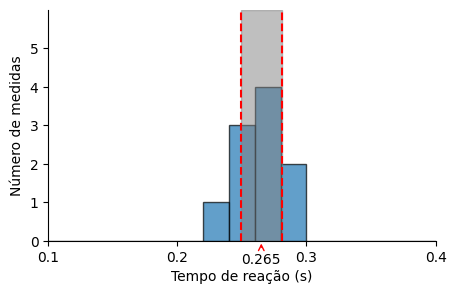
\includegraphics[width=0.92\linewidth]{histograma principal.png}
    \caption{A seta indica a posição e o valor da média no gráfico e as retas tracejadas delimitam o intervalo ocupado pelo desvio-padrão.}
    \label{histograma e dp}
\end{figure}


Na figura~\ref{dp alpha e beta} abaixo, vemos o gráfico com as médias e desvios-padrão dos dois grupos de medidas mostrados anteriormente na figura~\ref{consistência}. O grupo de medidas obtidas pela ``pessoa \textit{A}"  possui um desvio-padrão maior que o grupo da ``pessoa \textit{B}''. Ou seja, as medidas de \textit{B} estão menos dispersas (foram mais consistentes) que as medidas de \textit{A}.

\begin{figure}[H]
    \centering
    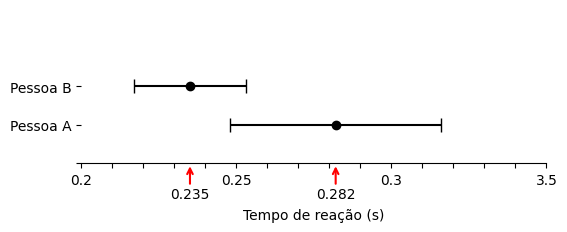
\includegraphics[width=0.95\linewidth]{pessoas alpha e beta.png}
    \caption{Representação gráfica da média e desvio-padrão do tempo de reação de duas pessoas \textit{A} e \textit{B}.}
    \label{dp alpha e beta}
\end{figure}

Os desvios-padrão permitem responder a perguntas interessantes. Por exemplo, vemos que o tempo de reação médio de \textit{B} é menor do que o de \textit{A}. Entretanto, se essas duas pessoas medirem mais uma vez seus tempos de reação, é possível que nesse caso o tempo de \textit{A} seja menor que o de \textit{B}? A figura~\ref{dp alpha e beta} sugere que a resposta é sim, é possível. Como há uma interseção entre os intervalos dados pelo desvio-padrão das duas pessoas, é possível que uma particular reação de \textit{B} seja mais lenta que uma de~\textit{A}. Contudo, considerando a pequena interseção entre os intervalos, essa inversão será pouco provável.

\section{Flutuação da média e desvio-padrão da média}

Já sabemos como representar um conjunto de medidas, pela sua média, e como medir sua dispersão, pelo desvio-padrão. Entretanto, para a realização de comparações, temos que saber o quão precisa é a nossa representação pela média do objeto em questão (no caso, o tempo de reação). Note que se repetíssemos a realização de dez medições, como as discutidas na seção 4, os resultados individuais não seriam exatamente os mesmos da tabela \ref{tab:widgets}. Por isso, é provável que a média das dez novas medidas, feitas pela mesma pessoa, seja diferente da anterior. A figura~\ref{duas tomadas} mostra o histograma e a média das dez medidas que apresentamos na seção 4. Ao lado, está o histograma de outras dez medidas feitas pela mesma pessoa. Note que os dois histogramas são diferentes e que, consequentemente, as médias não são idênticas.

\begin{figure}[H]
    \centering
    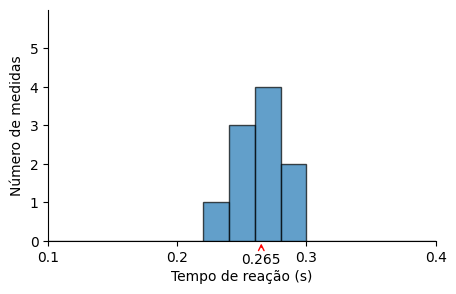
\includegraphics[width=0.48\linewidth]{histograma princ..png}
    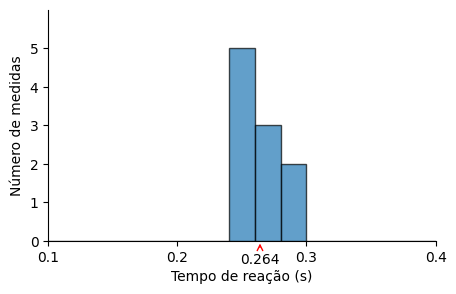
\includegraphics[width=0.48\linewidth]{segunda tomada.png}
    \caption{ Dois grupos de dados obtidos pela mesma pessoa. As médias de cada grupo estão indicadas pelas setas}
    \label{duas tomadas}
\end{figure}

Como diferentes grupos de medidas da mesma quantidade podem ter médias diferentes, isso significa que há uma incerteza associada à média. Para avaliar a variação da média, a pessoa que obteve as medidas da figura~\ref{duas tomadas} realizou mais oito conjuntos de dez 
medições e anotou o valor das médias obtidas em cada conjunto na tabela~\ref{tabela médias}.

\begin{table} [H]
\centering
\begin{tabular}{l|r}
Conjunto & Média (s) \\\hline
1 & 0,265 \\
2 & 0,264 \\
3 & 0,262 \\
4 & 0,261 \\
5 & 0,275 \\
6 & 0,267 \\
7 & 0,258 \\
8 & 0,260 \\
9 & 0,264 \\
10 & 0,265\\
\end{tabular}
\caption{\label{tabela médias} Médias dos conjuntos de dez medidas. Os histogramas dos conjuntos 1 e 2 são aqueles mostrados na figura~\ref{duas tomadas}.}
\end{table}

A distribuição dessas médias está mostrada na figura~\ref{histograma das médias}. Vemos que o histograma das médias é bem mais estreito do que os histogramas de medidas individuais apresentados na figura~\ref{duas tomadas}.
 
\begin{figure}[H]
    \centering
    \includegraphics[width=0.6\linewidth]{histograma das médias.png}
    \caption{Histograma com os dados presentes na tabela~\ref{tabela médias}. Oito das dez médias estão entre 0,26~s e 0,27~s}
    \label{histograma das médias}
\end{figure}



 Quanto maior o número $n$ de medidas, mais precisa (menos incerta) será a média. Caso tomemos as médias de dez conjuntos com cem medidas do tempo de reação da mesma pessoa em cada, essas dez médias serão ainda mais próximas entre si do que as médias de conjuntos de dez medidas mostradas na figura~\ref{histograma das médias}. A estabilização do valor médio com o aumento do número de medidas pode ser atribuída ao ganho de informação sobre o objeto medido. Para um conjunto de $n$ medidas, a incerteza da média é dada pelo \textbf{desvio-padrão da média}~$\sigma_M$, também chamado de \textbf{erro-padrão}.

Pode-se demonstrar que o erro-padrão de um conjunto com $n$ medidas é dado por

\[\sigma_M=\frac{\sigma}{\sqrt{n}}\, ,\]
onde $\sigma$ é o desvio-padrão das medidas, discutido na seção 5. O intervalo entre $\Bar{t} - \sigma_M$ e $\Bar{t} + \sigma_M$ nos fornece onde a média de um novo grupo de $n$ medidas provavelmente será encontrada.
Utilizando os dados fornecidos na tabela~\ref{tab:widgets}, temos o seguinte erro-padrão:

\[\sigma_M = \frac{0,016}{\sqrt{10}}=0,005\, .\]
Com isso o intervalo de $\Bar{t}-\sigma_M$ até $\Bar{t}+\sigma_M$ vai de 0,260 a 0,270~s. É fácil verificar que esse intervalo contém 8 das 10 médias presentes na tabela~\ref{tabela médias}. 

Portanto, mais medidas levam à diminuição do erro-padrão e do intervalo de incerteza na média. Isso está ilustrado na figura~\ref{ganho de precisão}, que mostra o efeito do aumento do número $n$ de medidas sobre a representação final dos dados. 
Nela estão marcados a média e o erro-padrão para as nossas medidas originais ($n=10$) e os para os valores obtidos com $n=50$ e $n=100$.  

\begin{figure}[H]
    \centering
    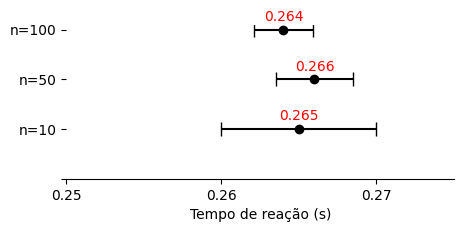
\includegraphics[width=0.7\linewidth]{n - 10, 50, 100.png}
    \caption{O tempo de reação médio de uma pessoa obtido com diferentes números de medidas. As barras representam o erro-padrão.}
    \label{ganho de precisão}
\end{figure}

Um ponto a ser ressaltado é que, ao contrário do erro-padrão $\sigma_M$, o desvio-padrão $\sigma$ tende a se estabilizar quando o número de medidas aumenta. 
O desvio-padrão indica a dispersão das medidas individuais, enquanto o erro-padrão indica a nossa confiança sobre a média.

\section{Comparações entre grupos de dados}

Para lidar com comparações entre grupos de dados, vamos olhar para a figura~\ref{A e B vert}. Nela, posicionamos verticalmente o eixo que informa o tempo de reação, pois esse estilo gráfico é mais comum do que aquele que vínhamos utilizando. Temos as médias dos tempos de reação das pessoas \textit{A} e \textit{B}, já apresentadas anteriormente na seção~5 (figura~\ref{consistência}), desta vez com as barras de erro-padrão. Olhando para as informações no gráfico, é possível afirmar que uma das duas pessoas tem, em média, reação mais rápida?

\begin{figure}[H]
    \centering
    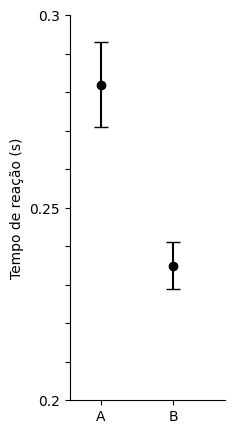
\includegraphics[width=0.22\linewidth]{volta de A e B vert.png}
    \caption{Médias e barras de erro-padrão de 10 medidas de tempo de reação das pessoas \textit{A} e \textit{B}.}
    \label{A e B vert}
\end{figure}

Pela figura, parece claro que \textit{A} tem um tempo de reação médio maior que \textit{B}. Um detalhe importante para essa conclusão é a observação das barras de erro-padrão. Elas mostram a incerteza das médias e vemos que há um grande espaço (vão) entre o limite inferior da barra de \textit{A} e o limite superior da barra de \textit{B}. É por conta disso que podemos afirmar que os tempos médios de \textit{A} e \textit{B} são diferentes: a probabilidade de encontrar uma diferença tão grande por mero acidente é muito pequena. Note que sem a informação dada pelas barras de erro não teríamos noção de quão imprecisas são as médias e quais valores poderiam ser encontrados caso fizéssemos outras medidas e obtivéssemos novas médias de \textit{A} e \textit{B}.

Vamos agora comparar duas outras pessoas, \textit{C} e \textit{D}. Na figura~\ref{C e D} vemos um gráfico parecido com o anterior. Temos as médias das medidas do tempo de reação de \textit{C} e \textit{D}, junto das suas barras de erro-padrão. Olhando para o gráfico, é possível afirmar que uma dessas pessoas tem, em média, reação mais rápida?

\begin{figure}[H]
    \centering
    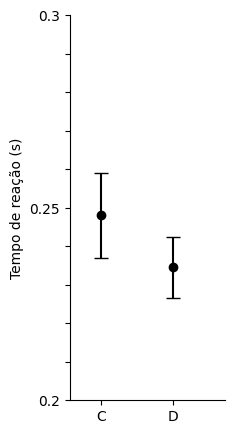
\includegraphics[width=0.22\linewidth]{C e D.png}
    \caption{Médias e barras de erro-padrão de 10 medidas de tempo de reação das pessoas \textit{C} e \textit{D}.}    \label{C e D}
\end{figure}

Como na figura anterior, as médias possuem valores diferentes. Contudo, temos uma situação em que não há vão entre as barras, há inclusive uma sobreposição entre elas. Os dados do gráficos não nos permitem \textbf{garantir} que os tempos de reação médios de \textit{C} e \textit{D} são diferentes. A sobreposição entre as barras indica que se fizéssemos outras medidas e obtivéssemos novas médias, essas novas médias poderiam resultar até em uma inversão de ordem entre \textit{C} e \textit{D}.


Podemos generalizar o raciocínio que nos levou às conclusões acima com algumas ``regras de bolso": 

\smallskip

\begin{itemize}
\item Quando o vão entre as barras de erro-padrão de duas médias a serem comparadas tem o comprimento de aproximadamente um erro-padrão, podemos dizer que há uma \textbf{probabilidade razoável de existir uma diferença} entre as quantidades representados pelas médias. A figura~\ref{regra única} mostra a situação em que o vão tem comprimento de um erro-padrão.
\end{itemize}

\begin{figure}[H]
    \centering
    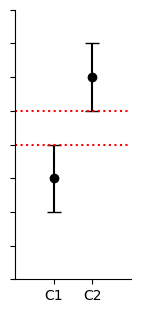
\includegraphics[width=0.25\linewidth]{regra 2.1.png}
    \caption{Comparação entre as médias de dois conjuntos de medidas, \textit{C1} e \textit{C2}. A distância entre cada traço no eixo vertical equivale a um erro-padrão.}
    \label{regra única}
\end{figure}

\smallskip

\begin{itemize}
\item Se há interseção entre as barras dos dois conjuntos de medidas ou se o vão tem comprimento bem menor que um erro-padrão, então \textbf{os dados não permitem afirmar que há uma diferença} entre as quantidades que comparamos. A figura~\ref{regra 1} traz gráficos que ilustram essas situações.
\end{itemize}

\begin{figure}[H]
    \centering
    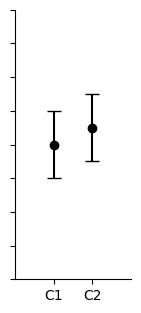
\includegraphics[width=0.22\linewidth]{regra 1.1.png}~
    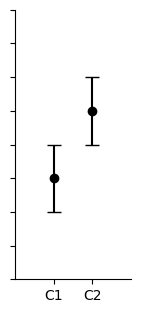
\includegraphics[width=0.22\linewidth]{regra 1.2.png}~
    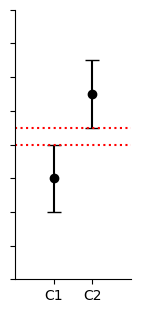
\includegraphics[width=0.22\linewidth]{regra 1.3.png}
    \caption{Situações em que os dados não permitem afirmar que há uma diferença entre as quantidades representadas pelas médias.}
    \label{regra 1}
\end{figure}

\smallskip

\begin{itemize}
\item Caso o vão seja bem maior que um erro-padrão, podemos afirmar que \textbf{é praticamente certo que haja uma diferença} entre as quantidades que estamos comparando. Essa situação está ilustrada na figura~\ref{regra 2}. 
\end{itemize}

\begin{figure}[H]
    \centering
    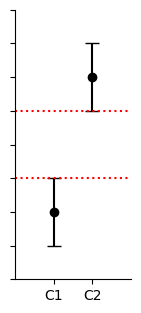
\includegraphics[width=0.23\linewidth]{regra 2.2.png}
    \caption{Vão com o comprimento de dois erros-padrão.}
    \label{regra 2}
\end{figure}

\smallskip

\begin{itemize}
    \item Na situação em que lidamos com médias que possuem \textbf{erros-padrão diferentes}, aplicamos as regras de bolso comparando o vão entre as barras ao maior dos erros-padrão.
\end{itemize}

A regra correspondente à figura~\ref{regra 2} se aplica às medidas de tempo de reação mostradas na figura~\ref{A e B vert}, e foi assim que concluímos que o tempo de reação da pessoa \textit{A} deve se maior que o da pessoa \textit{B}, estando praticamente certos disso.

É importante ressaltar que esse tipo de comparação não nos permite afirmar que duas quantidades são iguais. Só podemos dizer que elas são (muito provavelmente) diferentes, ou que não podem ser diferenciadas a partir dos dados disponíveis. Quando duas grandezas não podem ser diferenciadas, como nas situações da figura~\ref{regra 1}, isso não significa que elas sejam iguais.

\end{document}